\chapter{Introduction to Flexibility Management and The Goal of This Thesis}
\label{ch:introduction}
%\input{introduction}
\section{Defining flexibility and flexibility management}
Maintaining balance between supply and demand is a fundamental requirement to electric power system operations. The capability of a power system to match the supply and demand at each point of time by using control resources are often referred to as ``operational flexibility", or simply ``flexibility" \cite{Cochran2014,Wang2017,Lund2015,Delft}. Flexibility is therefore not a new concept. Power systems are inherently with uncertainty and variability since loads vary over time and occasionally in unexpected ways, and power plants may suffer unpredictable failures sometimes. All power systems are designed and built with certain level of flexibility to cope with those unexpected events. Conventionally, the flexibility is mainly enabled on the supply side, where dispatchable resources are controlled to adjust their outputs to match the time-varying load.

However, following radical transformations towards decarbonization, decentralization and digitalization in the energy industry, the existing operating model of electricity flexibility is being critically challenged and increasing interests are moving to flexibility from the load side and energy storage technologies\cite{Lund2015,Bronski2015,McKinsey&Company2010}. These disruptions are not only in technological but also in institutional and managerial manners, which are sparking market restructures and business model innovations. For instance, those new resources are typically smaller in scale compared the traditional flexible generations so the new operating model shall be managed via more decentralized approaches. Flexibility management, as an emerging business term, refers to the process how those new small-to-medium scale sources of flexibility are enabled, organized and exploited to serve the needs of power systems.

\section{Challenges in power system flexibility}

The penetration of renewable energy sources (RES), which is spreading over the whole industry globally \cite{Agency2016}, are commonly viewed as the fundamental driver for the transformation that is creating operational challenges in maintaining system balance with existing flexibility resources \cite{Cochran2014,Wang2017,Lund2015,FraunhoferIWES2015,Muller2016,Kwon2014,Kondziella2016,Papaefthymiou2016,Alizadeh2016,Bertsch2016}. The impacts of RES on electric power systems can be deduced from the instinct technological attributes of RES \cite{Kondziella2016,Edenhofer2013}:
\begin{itemize}
	\item RES is variable and often viewed as non-dispatchable since its output is determined by weather conditions, and furthermore
	\item RES is usually imperfectly predicted and specific power generation is uncertain until realization.
\end{itemize}

Effects of the property being non-dispatchable can be illustrated by introducing the concept of ``net load", also referred to as ``residual load", which equals the total system load minus the renewable generation so represents the load that needs to be served by non-RES resources\cite{Cochran2014,Muller2016,Ueckerdt2015}.

\begin{figure}[h!]
	\centering
	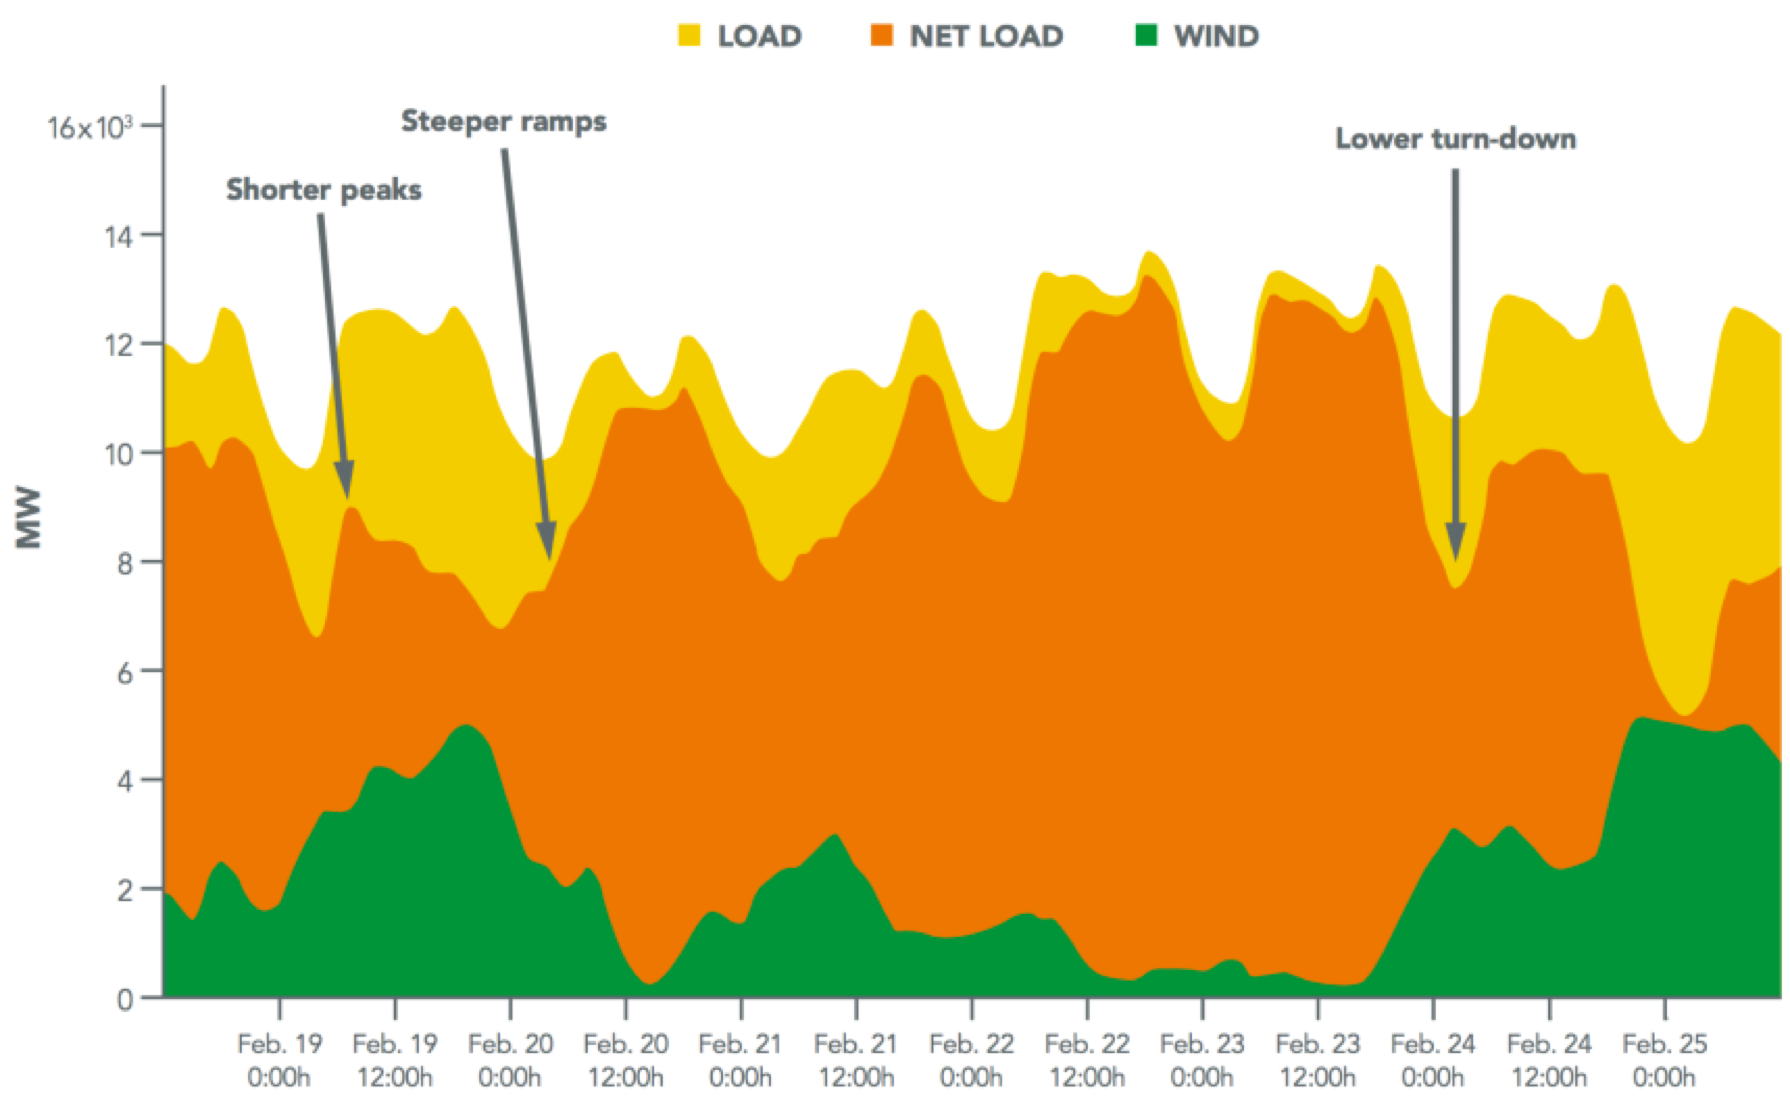
\includegraphics[width=0.9\linewidth]{Figures/NetLoad}
	\caption{An illustrative example of net load profile \cite{Cochran2014}}
	\label{fig:net-load}
\end{figure}

Figure \ref{fig:net-load} shows an example profile of net load, based on which we can see how RES is stressing the existing non-RES generations:

\begin{itemize}
	\item \textbf{Shorter peaks}: resulting in fewer operating hours for conventional peak generators, affecting their cost recovery and consequently long-term security of supply,
	\item \textbf{Lower turn-down}: diminishing the base load which was stable at a higher without RES, creating challenges to base generators who have limit operational flexibility to vary their outputs, and
	\item \textbf{Steeper ramps}: demanding higher performance in delivering flexibility, eliminating relative low-grade resources from serving the needs for flexibility.
\end{itemize}

It can be seen that the whole span of current generation portfolio serving base, flexible and peak power is under great pressure with the RES growth.

The issue of the forecast error, on the other hand, requires the dispatch of flexibility close to real-time operation. This is especially an explicit issue in places where those activities are organized through power markets. In present power markets, the major part of the scheduling and pre-dispatching is determined ahead of the operating day based on forecasts and errors deviated in real time from the schedule are mostly depending on imbalance settlements via so-call frequency control ancillary services which are typically more costly\cite{Ranci2013,Srivastava2011}. The intra-day market with higher resolution of price signals and shorter prediction horizon toward actual operation is a feasible option and implemented in many markets\cite{Srivastava2011} but intra-day markets are empirically prone to low liquidity \cite{Lund2015, Hagemann2015}. Without structural improvements in the market design, the demands for frequency control services would raise significantly and thus add burdens to the power system operators \cite{GEEnergyConsulting2014,Krad2017}. Many feasible solutions have been proposed \cite{Woo2016,Gonzalez-Aparicio2015,Koch2009,Weber2010,Wartsila2014} but market restructure is a complicated manner and may disrupt existing businesses.

Besides, solar power which is forecasted to have even higher potential than wind power in the long run is tending to grow in distributed patterns \cite{Agency2016,Epia2016,Sawyer2016}. With the conventional centralized deployment of flexibility, local congests are likely to deteriorate \cite{Lund2015,STEINKE2013826} which drives the needs for extensions of transmission and distribution capacity.

Collectively, the RES penetrations urge innovations in both technology and market design, which are otherwise burdening power system operators with higher expenses, potentially reducing the revenue scream of existing market players and/ or leading to significant curtailment of RES.

In addition to RES, the electrification of transportation, i.e. the penetration of plug-in electric vehicles (EV), is emerging more recently to be a second pole as the game changer. Facilitated by support policies by states or cities to uncap their multiple benefits such as transport decarbonization, air pollution reduction, and energy efficiency and security, the growth of EV has been accelerating significantly, having exceeded the global threshold of 2 million in 2016 \cite{InternationalEnergyAgency2017}. Although it tends to be treated as a promising source for flexibility by implementing vehicle to grid (V2G) technologies \cite{Size2016,Habib2015,Foley2013}, threats along with it shall not be ignored. Without being fully prepared in technologies and markets, the growth of EV may still move to the opposite side of flexibility with the negative impacts such as increasing peak demand and potential local congestion \cite{Green2011,DBLP:journals/corr/PournarasJZFS17}.

It has been pointed out that lack of flexibility can be identified more intuitively by signals such as \cite{Cochran2014,Wang2017}:
\begin{itemize}
	\item difficulty balancing demand and supply, resulting in frequency excursions or shedded load,
	\item significant renewable energy curtailments,
	\item negative market prices, and
	\item high price volatility in whole power markets.
\end{itemize}

Although having been discussed extensively for years in the academic area and by industry experts, it was not until quite recently when more and more signs of inflexibility had been witnessed did most of the public start to be indeed aware of the challenges on power system flexibility. For instance, the negative pricing in wholesale power spot market was first introduced in 2007 in Germany intra-day market and in 2008 in Germany/Australia day-ahead market\cite{EPEX_negative_price}, but vast attentions from the public were initiated after 146 hours on 24 days with negative prices were observed in the day-ahead market in 2017. Another famous example could be the power outage in South Australia that happened on September 28th 2016. After a widespread debate, Australia Energy Market Operator (AEMO) finally concluded in its investigation report that the generation deficit of wind farms due to unexpected operations of a control setting responding to multiple disturbances led to the power blackout  \cite{AEMO2016SA}.  This aroused public's worries on supply security from RES generation. As one of the follow-up actions, AEMO partnering with Tesla Inc., one of the leaders in global battery and electric vehicle markets,  built the worlds' largest battery energy storage system (BESS) in South Australia \cite{AEMO_tesla}.

These imply a proper timing for technology vendors to update their assessment on the market, as interests in flexibility management from the public and thus their potential customers have significantly raised.

\section{Technologies: options for system flexibility provision}

Many different resources are available to deliver grid flexibil- ity. Flexibility can come from physical assets such as batteries and fast-ramping gas plants, but it can also come from improved operations, such as shorter dispatch intervals, new ancillary ser- vices, and improved weather forecasting [75]. In general, the lowest cost options fall into the category of improved grid oper- ations due to the fact that it can utilize the existing infrastructure and make relatively small operational changes to efficiently bal- ance the energy demand and supply. Other options, as shown in Fig. 1, are available but relatively more expensive than im-proved operations [76]. In what follows, literature on different approaches is briefly introduced.
1) Improved Operations: Advanced models and algo- rithms for improving the UC and ED processes are in the cen- tral of operational improvements. For instance, tight and com- pact mixed-integer linear programming (MILP) formulation has been proposed to model the startup (SU) and shutdown (SD) power trajectories of thermal units [77] and the configuration of combined-cycle units [78]. Improving the wind, solar, and load forecasting is another approach to enhance power system operational flexibility [30].
2) Demand Response: Incorporating dispatchable de- mand response resources (DRRs) into the energy market can in- crease the grid flexibility. In MISO, DRRs can bid into the ancil- lary service to provide regulation services [79, old82], while in Electricity Reliability Council of Texas (ERCOT) the DRRs are heavily utilized to provide spinning reserves [80]. The emerg- ing demand response techniques include the smart thermostats, building automation systems, plug-in EVs, and others.
3) Improved Grid Infrastructure: Transmission conges- tion is a major bottleneck for delivering flexible power in the grid. Increased transmission capacity can facilitate the electric- ity delivery within or among balancing areas, thus help balance the supply and demand. On the distribution side, the implemen- tation of large volume of sensors and smart meters, communi- cation devices, and advanced information technologies can also help balance out supply and demand.
4) Fast Start Resources: In real-time operations, fast start resources such as combined-cycle units, aero-derivative gas turbines, and reciprocating engine turbines have short start up time and rapid ramp rates, thus can provide needed system flexibility [81].
5) Energy Storage: An abundance of energy storage (ES) technologies including grid-scale batteries, pumped hydro, com- pressed air, fly wheel and others can provide flexibility on the grid [82]. \cite{Wang2017}




\begin{figure}[h!]
	\centering
	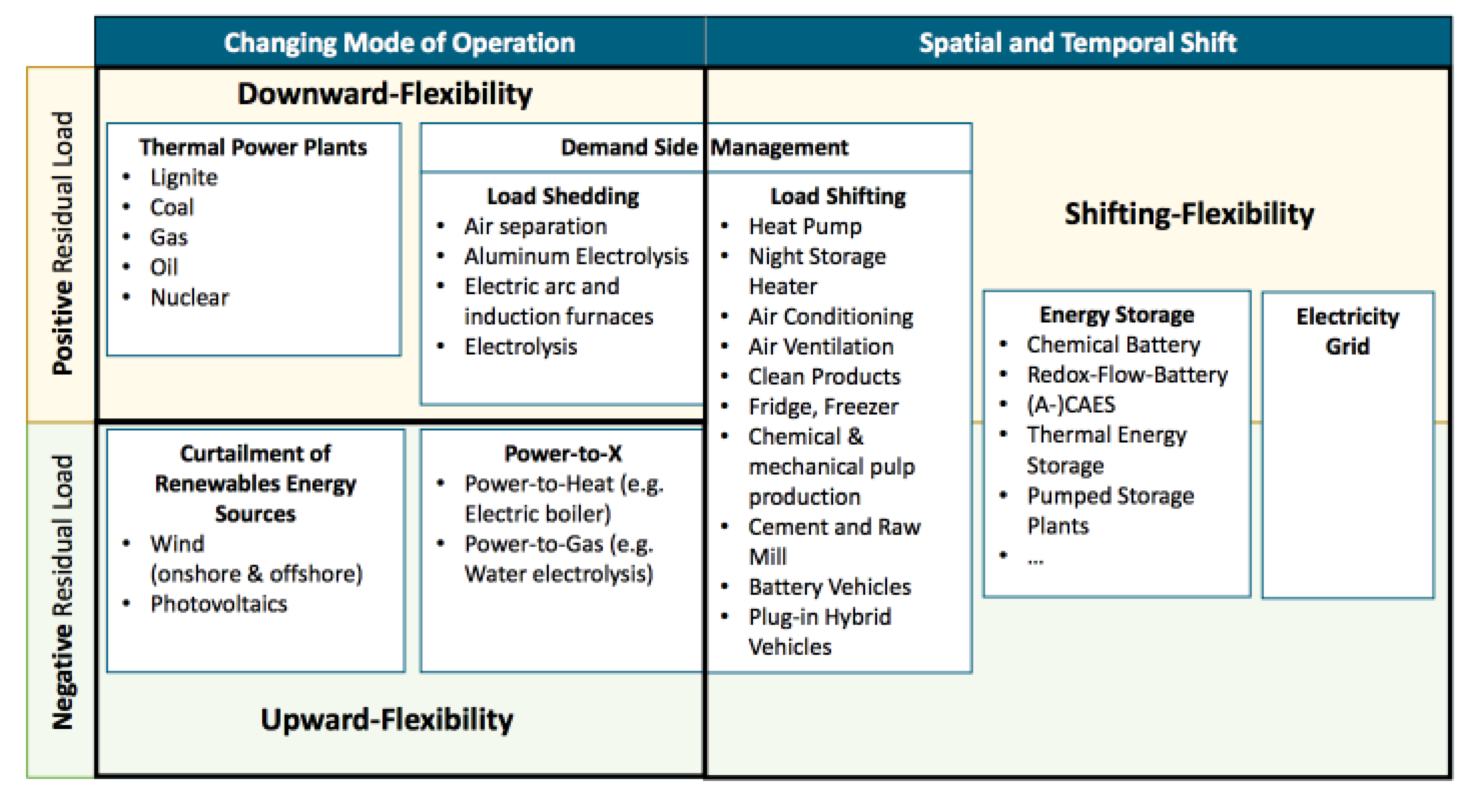
\includegraphics[width=0.95\linewidth]{Figures/TechnologyOptions}
	\caption{Overview flexibility options categorized in way of flexibility provision \cite{Muller2016}}
	\label{fig:TechnologyOptions}
\end{figure}

\section{Applications, benefits and business models}
\subsection{In liberalized market}


(placeholder)
\newpage
(placeholder)
\newpage
(placeholder)
\newpage
(placeholder)
\newpage

%\subsubsection{Needs of different plyaers}

Player * Market * Application


%\subsubsection{Energy Markets}


%\subsubsection{Ancillary Service Markets}

\subsection{In vertically integrated market}
(placeholder)
\newpage


\section{Scope and research questions}

The target audience of this thesis is the management at Landis+Gyr on a high coporate level.

The ultimate goal is to provide references to support the audiences' strategic decision makings regarding flexibility management.

In order to achieve this, we conducted qualitative studies and developed quantitative models to identify: 1) the value of markets for flexiblity management

\begin{itemize}
	\item 
\end{itemize}

The goal of this thesis is to:

developed a robust modeling tool with moderate complexity so that it can not only provide results in current environment but can be also reused or easily revised to provide results in case of changes in the future.

based on the tool, make quantitative as well as quanlitative analysis to provide refer 

Purpose: providing references for strategic decision makings regarding flexibility management.

In order to make the analysis robust and reliable, we have built a techno-economic models which include the bottom-up dynamics of some key elements regarding the electricity markets and flexilibity technologies. 

However, it shall be noticed this thesis is not intended to serve for:

project developers to design a flexiblity system or make operating (including bidding) strategies of the system

policy makers to redesign the electricity market structure, rules or other policies

grid planners to understand the needs and options of flexibility in order to acheive system relability with lowest costs


Since the concept of flexiblity management is related to a great variety of technologies, applications and Landis+Gyr is positioning globally in various markets, the scope could be very broad. Nonetheless, in order to produce viable and reliable results with a solidily established techno-economic model, we have to make comprises. According to the relevance to Landis+Gyr's business, the scopes are defined as:

%\subsection{Scope of technologies}

%\subsection{Scope of applications}

%\subsection{Scope of benefits and business models}
The potential business model of Landis+Gyr is either to supply products to the customers to help them enable flexibility or to directly sell them flexible MWs as a service. In this case, we want to understand the value of each MW we enabled or sold. We assume Landis+Gyr will not directly partipate and trade in the power market, as it is going to place Landis+Gyr at the rival side of some customers in that market.

The value of flexibility will definitely vary according to the purpose, users' portfolio and operating strategies. 


%\subsection{Scope of markets}